\fontfamily{\sfdefault}\selectfont
% XCircuit output "discrete_pll.tex" for LaTeX input from discrete_pll.ps
\def\putbox#1#2#3#4{\makebox[0.00000in][l]{\makebox[#1][l]{}\raisebox{\baselineskip}[0.00000in][0.00000in]{\raisebox{#2}[0.00000in][0.00000in]{\scalebox{#3}{#4}}}}}
\def\rightbox#1{\makebox[0.00000in][r]{#1}}
\def\centbox#1{\makebox[0.00000in]{#1}}
\def\topbox#1{\raisebox{-0.60\baselineskip}[0.00000in][0.00000in]{#1}}
\def\midbox#1{\raisebox{-0.20\baselineskip}[0.00000in][0.00000in]{#1}}
   \scalebox{1}{
   \normalsize
   \parbox{6.88333in}{
   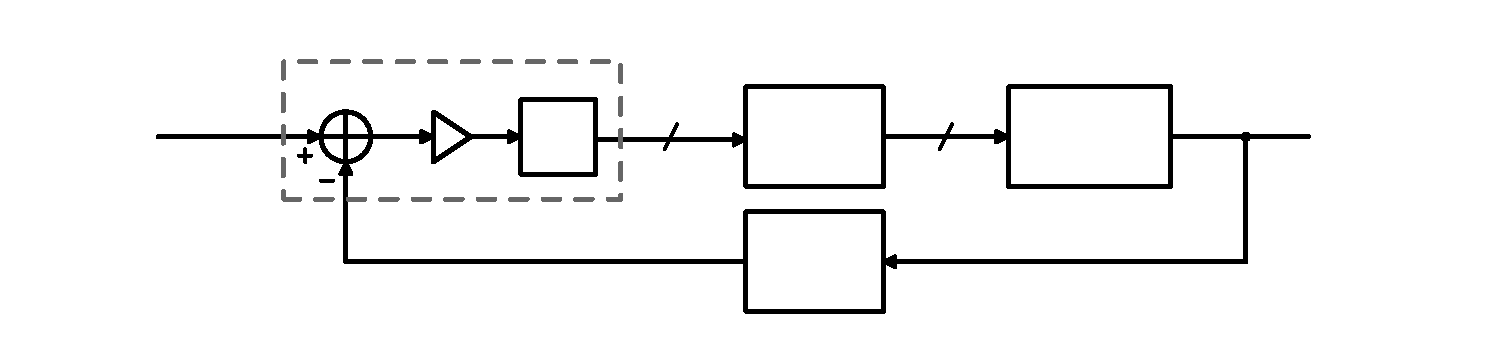
\includegraphics[scale=0.70000]{./figs/discrete_pll.pdf}\\
   % translate x=512 y=508 scale 0.38
   \putbox{0.74200in}{1.04300in}{1.20}{$\Phi_{ref}$[n]}%
   \putbox{2.17000in}{0.47600in}{1.20}{$\Phi_{div}$[n]}%
   \putbox{3.00300in}{1.07800in}{1.20}{e$_\Phi$[n]}%
   \putbox{2.06500in}{1.12000in}{1.20}{\rotatebox{-360}{$\frac{\mathrm{M}}{2\pi}$}}%
   \putbox{1.75700in}{1.04300in}{1.20}{$\Phi_e$}%
   \putbox{2.47800in}{0.91700in}{1.20}{$\lfloor x\rfloor$}%
   \putbox{1.32300in}{1.36500in}{0.90}{TDC}%
   \putbox{3.55600in}{0.91700in}{1.20}{H$_{LF}$(z)}%
   \putbox{4.28400in}{1.07800in}{1.20}{u[n]}%
   \putbox{4.73200in}{0.93100in}{1.20}{$\frac{2\pi K_{DCO}T}{1-z^{-1}}$}%
   \putbox{5.55100in}{1.04300in}{1.20}{$\Phi_{out}$[n]}%
   \putbox{3.62600in}{0.32900in}{1.20}{$\div$ N}%
   \putbox{4.70400in}{1.23200in}{0.90}{DCO}%
   } % close 'parbox'
   } % close 'scalebox'
   \vspace{-\baselineskip} % this is not necessary, but looks better
\fontfamily{\rmdefault}\selectfont
